\documentclass{article}
\usepackage{hyperref}
\usepackage{graphicx} % Required for inserting images

\title{Final Solution Report}
\author{Hokimiyon Muhammadjon}
\date{November 2023}

\begin{document}

\maketitle

\section{Introduction}
This report contain solution of Text De Toxification problem using Transformer. Solution consist of 4 parts:
\begin{enumerate}
    \item Data processing
    \item Define architecture
    \item Training process
    \item Results
\end{enumerate}

\section{Data analysis}
Dataset consist of 6 features: 
\begin{itemize}
    \item reference $\mapsto$ Toxic sentence
    \item ref\_tox $\mapsto$ Toxicity level of reference text
    \item translation $\mapsto$ Paraphrase version of the reference
    \item trn\_tox $\mapsto$ toxicity level of translation text
    \item similarity $\mapsto$ cosine similarity of the texts
    \item length\_diff $\mapsto$ relative length difference between texts
\end{itemize}
Target column is translation sentence. Our model read toxic sentence (reference column in our case) and predict less toxic sentence (translation column in our case).

First have to replace more toxic sentence in to reference column: there is case toxicity level of paraphrase version is higher than reference sentence. Then divide abbreviations in to original form (I'm $\mapsto$ I am). after that apply word\_tokenize. Also applied spelling correction (livt $\mapsto$ live).

\section{Define architecture}
The architecture named Transformer. 

Transformer architecture:

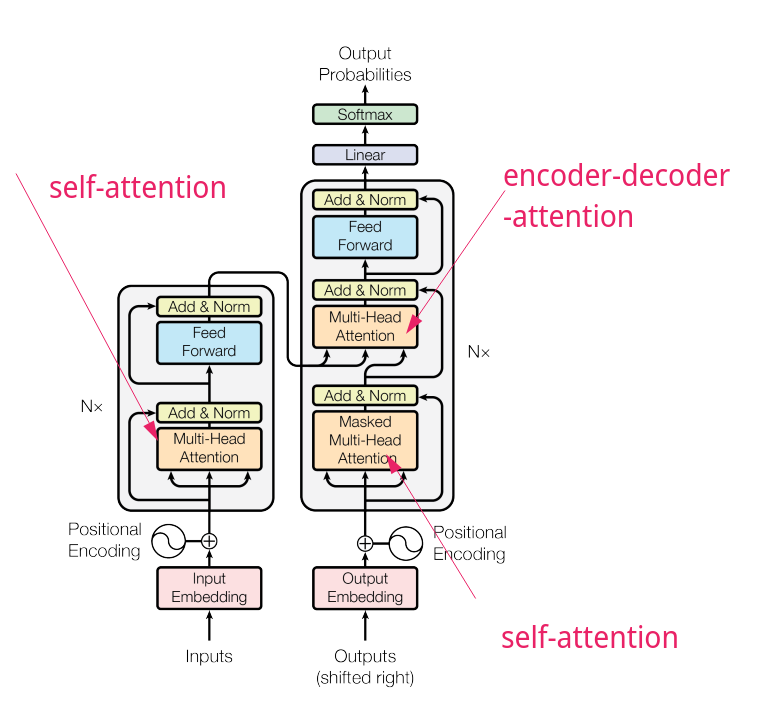
\includegraphics[scale=1.0]{figures/Transformer.png}

Transformer consist of encoder and decoder parts.

Encoder: The input sequence is fed into the encoder, which consists of multiple identical layers. Each layer has two main subcomponents: a multi-head self-attention mechanism and a feedforward neural network. The self-attention mechanism allows the model to consider different parts of the input sequence when encoding each element.

Decoder: The output sequence is generated by the decoder, which also consists of multiple identical layers. Each decoder layer combines self-attention and encoder-decoder attention mechanisms (as written in Attention section). The self-attention mechanism helps the decoder focus on different parts of the generated output sequence, while the encoder-decoder attention mechanism lets the model align the input and output sequences.

In transformer there is new part name Positional Encoding, because we don't use RNN type mechanism, we don't have information about positions, hence positional encodings are added to the input embeddings to provide the model with information about the position of each element in the sequence.

Also one more new part is feedforward Neural Networks: After applying attention mechanisms, each sublayer in the encoder and decoder includes a position-wise feedforward Neural Network to further process the information.

To stabilizing training and improving the flow of gradients through the deep network, the Layer Normalization and Residual Connections component introduced.

The parameters of model:
\begin{itemize}
    \item embed\_size = 512
    \item n\_layer = 6
    \item n\_head = 6
    \item hidden\_size = 512
    \item batch\_size = 128
    \item lr = 5e-5 $\mapsto$ for optimizer
    \item max\_lenght = 32
\end{itemize}

\section{Training process}
Training process of Transformer consist of several parts, first define loss function and optimizer.
\begin{description}
\item[Loss function:] CrossEntropyLoss
\item[Optimization Algorithm:] Adam
\end{description}
The training process for a Transformer model involves loading and batching preprocessed data, initializing model parameters, defining a loss function, selecting an optimization algorithm, and iterating over the dataset for a set number of epochs. In each training iteration, the model computes forward and backward passes, calculates gradients using the loss function, and updates parameters via the chosen optimization algorithm. Validation on a separate dataset is performed periodically to monitor performance, and save the model with best performance.

\section{Results}
Usually models generate output using greedy algorithm, but that algorithm not guarantee return the best result, hence in repository implemented $Beam$ $Search$ algorithm. $Beam$ $Search$ algorithm select first beam\_width best alternatives at each time until meet end of sentence, then return the best among them.

Examples of model:

\begin{itemize}
    \item origin $\mapsto$ original text
    \item translation $\mapsto$ translated text
    \item predicted $\mapsto$ the output of model
\end{itemize}

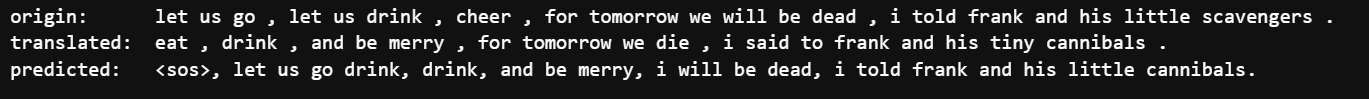
\includegraphics[scale=0.42]{figures/Transformer_result_1.png}

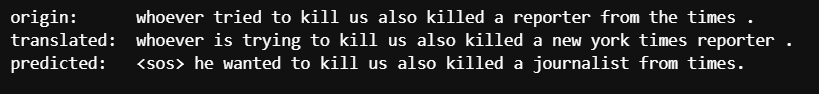
\includegraphics[scale=0.42]{figures/Transformer_result_2.png}

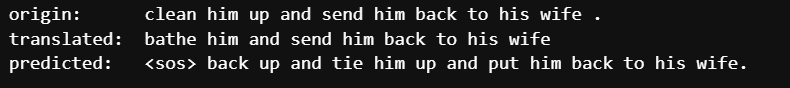
\includegraphics[scale=0.42]{figures/Transformer_result_3.png}

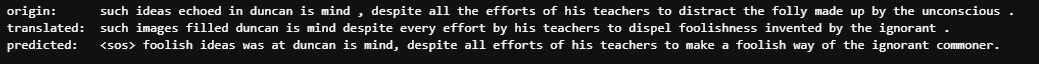
\includegraphics[scale=0.5]{figures/Transformer_result_4.png}

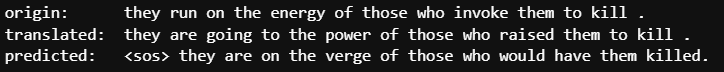
\includegraphics[scale=0.45]{figures/Transformer_result_5.png}

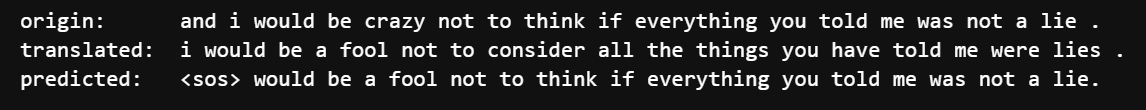
\includegraphics[scale=0.42]{figures/Transformer_result_6.png}



\begin{thebibliography}{1}

\bibitem{Transformer}
Vaswani, A. et al. (2017) \emph{Attention is All You Need}, In Advances in Neural Information Processing Systems, Vol. 30. [\href{https://papers.nips.cc/paper_files/paper/2017/hash/3f5ee243547dee91fbd053c1c4a845aa-Abstract.html}{link}]

\end{thebibliography}

\end{document}
